\chapter{A functional definition of analogical classifiers}
\label{CHAP:functional_definition}

\initial{I}n Section \ref{SEC:machine_learning_with_boolean_proportions}, we
briefly described a basic process of analogical classification in an unformal
way, making sure that everything went smoothly. In practice, bad things happen,
always. In this chapter, we will clearly and formally define analogical
classification, which will help us clarify some of the grey areas of Section
\ref{SEC:machine_learning_with_boolean_proportions}.

A first form of analogical classifiers has been defined in the works of Stroppa
and Yvon \cite{StrYvoCNLL05}, which we will refer to as \textbf{conservative
classifiers}. Another form of analogical classifiers has later been proposed in
the works of Bayoudh, Delhay and Miclet \cite{MicBayDelJAIR08,
BayMicDelIJCAI07}, refered-to here as \textbf{extended classifiers}.

Though the theoretical groundations of the conservative and extended
classifiers have a lot in common (they are both analogical classifiers after
all), we will see that their practical implementation are actually quite
different. We will show however that the extended classifier is a
generalization of the conservative one, and most importantly that these two
approaches can be factorized into a single, unifying framework.

So far, only algorithmic descriptions of both methods were available. Our
unifying framework will allow us to give a general and \textbf{functional}
definition of analogical classifiers, opening the door to some theoretically
grounded research.

\section{Analogical classification}

Let us first define the problem of classification, one of the main subfields of
machine learning. The aim is simple: a classifier has to estimate the class of
any element given as input on the basis of some other elements for which the
class is known. Formally, we denote $X$ our universe which is usually a
Cartesian product of dimension $m$: $X = X_1 \times X_2 \times \ldots \times
X_m$. We have at our disposal a subset $S \subsetneq X$ of $n$ pairs
$\left(\mathbf{x}, f(\mathbf{x})\right)$, called the \textbf{training set}.
$$S= \Set{\left(\mathbf{x}^{(i)}, f(\mathbf{x}^{(i)})\right) \in X^m \times Y |
i \in [1,n]}.$$

For any $\mathbf{x} \in X^m$, the value $f(\mathbf{x})$ is called its
\textbf{class} or \textbf{label}.
The functional notation $f(\mathbf{x})$ suggests that all labels
are defined by an underlying function $f \colon X^m \to Y$, which is the usual
general view point of machine learning. In the case of classification, $Y$ is a
finite set of size $C$ where $C$ is the number of different classes. The goal
of a classifier is to \textbf{learn} the function $f$ on the basis of the
elements in $S$, called the \textbf{examples}. The output of a classifier is a
function $\hat{f} \colon X^m \to Y$ that estimates the ground truth function
$f$. The estimated labels $\hat{f}(\mathbf{x})$ will also be denoted
$\hat{\mathbf{x}}$.

\subsection{Conservative classifier}
\label{SEC:conservative_classifier}

We will here describe what we call a \textbf{conservative} classifier. Without
further ado, let us consider Algorithm \ref{ALGO:conservative_classifier} which
describes conservative classifiers.

\begin{algorithm}[!ht]
\caption{The Conservative classifier}
\label{ALGO:conservative_classifier}
  \begin{algorithmic}
    \STATE {\bf Input}: A training set $S$ and an element $\mathbf{x} \in X^m
    \setminus S$ for which $f(\mathbf{x})$ is unknown.
    \STATE {\bf Output}: $\hat{f}(\mathbf{x})$, an estimation of
    $f(\mathbf{x})$
    \STATE {\bf Init}: $\mathbf{C}(\mathbf{x}) = \varnothing$ \quad \quad // A multiset of candidate
    labels.

    \FORALL{$(\mathbf{a}, \mathbf{b}, \mathbf{c}) \in S^3$ such that
    $\mathbf{a} : \mathbf{b} :: \mathbf{c} : \mathbf{x}$}
    \IF{$f(\mathbf{a}) : f(\mathbf{b}) ::f(\mathbf{c}) : y$ is
    solvable}
    \STATE $y = \sol\left(f(\mathbf{a}), f(\mathbf{b}), f(\mathbf{c})\right)$
    \STATE $ \mathbf{C}(\mathbf{x}) = \mathbf{C}(\mathbf{x}) \cup y$
    \ENDIF
	  \ENDFOR
    \STATE $\hat{f}(\mathbf{x}) = \text{Mode} (\mathbf{C}(\mathbf{x}))$ // The most common value in
    $\mathbf{C}(\mathbf{x})$ (undefined if $\mathbf{C}(\mathbf{x}) = \varnothing$).
  \end{algorithmic}
\end{algorithm}

It should be easy to see that the process of Algorithm
\ref{ALGO:conservative_classifier} is extremely similar to the one we followed
on our gentle introduction to classification with Boolean proportions in
Section \ref{SEC:machine_learning_with_boolean_proportions}. Here again the key
underlying process is the analogical inference principle, which states that if
four elements are in proportion, then their classes should also be in
proportion. But Algorithm \ref{ALGO:conservative_classifier} is slightly more
general than what we have glimpsed in Section
\ref{SEC:machine_learning_with_boolean_proportions}: it allows to deal with
cases where some of the candidate solutions $y$ do not agree with each other.
The fix here is to consider that the prediction $\hat{f}(\mathbf{x})$ will be
the most common candidate solution among all the predictors. This definition of
analogical classification comes from the work of Stroppa and Yvon
\cite{StrYvoCNLL05, StrYvoREPORT05}, and to our knowledge it is the first
instance of analogical learner that has every been proposed. We note however
that the authors did not explicitely state that the class equations must be
solvable to be useful.

Note that if the multiset $\mathbf{C}(\mathbf{x})$ is empty, i.e. if we cannot find
$3$-tuples in $S^3$ such that they are in proportion with $\mathbf{x}$ and such
that the related class equation is solvable, then the value
$\hat{f}(\mathbf{x})$  is undefined and $\mathbf{x}$ cannot be classified
(hence the name \textit{conservative}).

At first sight, we are here in a setting where the examples in $S$ are stored
for future use, without any generalization process.  We will thus consider (for
now) that the conservative classifier ranges among the category of
\textbf{lazy learners}, i.e. learners that only rely on the training set $S$
without any actual \textit{learning} stage, or without building any model of
the data. The most popular instance of lazy learner certainly is the famous
$k$-NN algorithm.

In the following, we will give a functional definition of $\hat{f}(\mathbf{x})$
as outputed by a conservative classifier. To this end, we will define two
crucial concepts: the \textbf{analogical extension} of a training set $S$, and
the \textbf{analogical root} of an element $\mathbf{x}$. Both the analogical
extension and the analogical root were first defined in \cite{StrYvoREPORT05},
with some minor differences with our definitions.

\begin{definition}
  \label{DEF:analogical_extension}
  Denoting $S$ a training set and $f$ the ground truth function of the labels,
  the \textbf{analogical extension} of $S$ using $f$ is:
  $$
  \esf \eqdef \Set{ \mathbf{x} \in X^m |  \exists
  (\mathbf{a},\mathbf{b},\mathbf{c}) \in S^3, ~ \mathbf{a} : \mathbf{b} ::
  \mathbf{c} : \mathbf{x} \emph{ and } f(\mathbf{a}) : f(\mathbf{b}) ::
  f(\mathbf{c}) : y \emph{ is solvable}}.
  $$
\end{definition}

Intuitively,  $\esf$ can be regarded as the set of all $\mathbf{x} \in X^m$
that are in proportion with at least one 3-tuple in $S$, provided that the
equation related to the associated labels is also solvable. For any $S$ and any
$f$, $\esf$ satisfies some interesting properties: \begin{enumerate}
\item $S \subseteq \esf$, since $\mathbf{x} : \mathbf{x} :: \mathbf{x}
  :\mathbf{x}$ always holds;
\item $\aext{\varnothing}{f} = \varnothing$, and $\aext{X^m}{f}=X^m$;
\item $S_1 \subseteq S_2 \implies \aext{S_1}{f} \subseteq \aext{S_2}{f}$.
\end{enumerate}

\begin{definition}
  \label{DEF:ae_star}
We will denote by $\esfs$ the set of elements in $\esf$ that are not in $S$:
$$\esfs \eqdef \esf \setminus S.$$
\end{definition}

\noindent
In a setting where for any $\mathbf{a},\mathbf{b}, \mathbf{c}$ the equation
$\mathbf{a} : \mathbf{b} :: \mathbf{c} : \mathbf{x}$ is always solvable (as is
the case for the arithmetic proportion) and such that the associated class
equation is also solvable, we can show that the size of $\esfs$ is exactly
$\frac{1}{2} n^2(n - 1)$. This value is thus a tight upper bound for $\mid
\esfs\mid$, because in practice equations are not always sovable.

To polish our understanding of the analogical extension, let us consider Figure
\ref{FIG:ae_example}.
\begin{figure}[!h]
\centering
  \includegraphics[width=3in]{figures/ae_example.pdf}
  \caption{With $S = \Set{\mathbf{a}, \mathbf{b}, \mathbf{e},
  \mathbf{g}}$, we have $\esfs\Set{\mathbf{f}, \mathbf{h}}$.}
\label{FIG:ae_example}
\end{figure}
The training set $S$ is $\Set{\mathbf{a}, \mathbf{b}, \mathbf{e},\mathbf{g}}$.
Taking $(\mathbf{a}, \mathbf{g}, \mathbf{b}) \in S^3$, we notice that
$\mathbf{a} : \mathbf{g} :: \mathbf{b} : \mathbf{h}$, and the associated class
equation $0:0::0:y$ is solvable. So $\mathbf{h} \in \esf$. The same goes for
$\mathbf{f}$ with the 3-tuple $(\mathbf{a}, \mathbf{e}, \mathbf{b}) \in S^3$.
However, even if we can find $(\mathbf{e}, \mathbf{g}, \mathbf{a}) \in S^3$
such that $\mathbf{e} : \mathbf{g} :: \mathbf{a} : \mathbf{c}$, the associated
class equation $1:0::0:y$ is not solvable, so $\mathbf{c} \notin \esf$. At
last, vertice $\mathbf{d}$ will suffer the same fate because the class equation
$f(\mathbf{e}) : f(\mathbf{b}) :: f(\mathbf{g}) : y$ is not solvable either. In
the end, $\esf = \set{\mathbf{a}, \mathbf{b}, \mathbf{e}, \mathbf{f},
\mathbf{g}, \mathbf{h}}$.

The dual concept of the analogical extension is what we call the
\textbf{analogical root} of a given element $\mathbf{x} \in X^m$:

\begin{definition}
  \label{DEF:analogical_root}
  Denoting $S$ a training set and $f$ the ground truth function of the labels,
  the \textbf{analogical root} of an element $\mathbf{x} \in X^m$ is:
  $$
  \rsfx \eqdef \Set{(\mathbf{a}, \mathbf{b}, \mathbf{c}) \in S^3 |
  \mathbf{a}:\mathbf{b}::\mathbf{c}:\mathbf{x} \emph{ and }
  f(\mathbf{a}):f(\mathbf{b})::f(\mathbf{c}):y \emph{ is solvable}}.
  $$
\end{definition}

$\rsfx$ is simply the set of 3-tuples in $S$ which are analogically linked to
$\mathbf{x}$. Considering again the example of Figure \ref{FIG:ae_example}, we have that
$\aroot{S}{f}{\mathbf{h}} = \Set{(\mathbf{a}, \mathbf{g},\mathbf{b}),
(\mathbf{a}, \mathbf{b},\mathbf{g})}$. However, the two related proportions
$\mathbf{a}: \mathbf{g}::\mathbf{b}:\mathbf{h}$ and $\mathbf{a}:
\mathbf{b}::\mathbf{g}:\mathbf{h}$ are equivalent, and we will follow the
convention that the analogical root should only contain non-equivalent
3-tuples, so technically $\aroot{S}{f}{\mathbf{h}}$ is entirely described by $\Set{(\mathbf{a},
\mathbf{g},\mathbf{b})}$.
We also have that $\aroot{S}{f}{\mathbf{f}} = \Set{(\mathbf{a}, \mathbf{e},
\mathbf{b})}$, $\aroot{S}{f}{\mathbf{a}} = \Set{(\mathbf{a}, \mathbf{a},
\mathbf{a})}$, and $\aroot{S}{f}{\mathbf{c}} = \varnothing$. It is clear that
in general,
$$\rsfx = \varnothing\iff \mathbf{x} \notin \esf.$$
\noindent
It should also be clear that even if we only consider unique 3-tuples (up to
equivalence) in the
analogical root, $\rsfx$ may contain more than one 3-tuple: for example in
$\mathbb{R}^m$ or $\mathbb{B}^m$ with the arithmetic (or Boolean) proportion,
$\mathbf{x}$ may be the involved in more than one parallelogram, as illustrated
in Figure \ref{FIG:multiple_parallelograms}.

\begin{figure}[!h]
\centering
  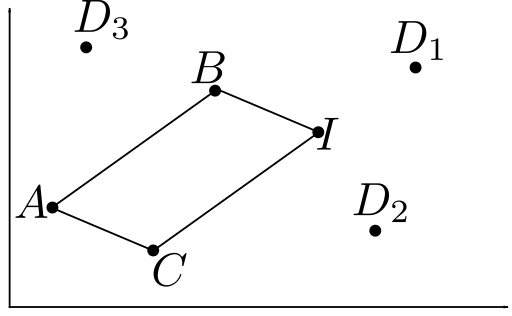
\includegraphics[width=2.5in]{figures/multiple_parallelograms.pdf}
  \caption{With $S = \Set{\mathbf{a}, \mathbf{b}, \mathbf{c}, \mathbf{a}',
  \mathbf{b}', \mathbf{c}'}$, we have $\mathbf{x} \in \esf$ and $\rsfx =
  \Set{(\mathbf{a}, \mathbf{b}, \mathbf{c}), (\mathbf{a}', \mathbf{b}',
  \mathbf{c}')}$. Class equations are all assumed to be solvable.}
\label{FIG:multiple_parallelograms}
\end{figure}

We need to introduce one last definition before we can go on with the
functional view of conservative classifiers:

\begin{definition}
  \label{DEF:analogical_label}
  For any element $\mathbf{x}$ of $\esf$, we denote $\mathbf{C}(\mathbf{x})$
  the set of the class equations solutions associated with $\mathbf{x}$:
  $$\mathbf{C}(\mathbf{x}) = \Set{y | f(\mathbf{a}) : f(\mathbf{b}) ::
  f(\mathbf{c}) :y~ \forall (\mathbf{a}, \mathbf{b}, \mathbf{c}) \in \rsfx}$$
  We then define the \textbf{analogical
  label} of $\mathbf{x}$ as:
  $$\albl{\mathbf{x}} \eqdef
  \begin{cases}
    f(\mathbf{x}) \emph{ if } \mathbf{x} \in S\\
    \text{Mode} \left(\mathbf{C}(\mathbf{x})\right) \emph{ if
    } x \notin S
  \end{cases}
  $$
  where $\text{Mode}(\mathbf{C})$ returns the most frequent element of the multiset
$\mathbf{C}$. In case of a tie, the returned element is chosen at random between
the most frequent elements.
\end{definition}

We are now in position to give a functional definition of the conservative
classifier:

\begin{definition}
  \label{DEF:conservative_classifier}
  Given a training set $S$ with an underlying ground truth function $f$,
  a conservative classifier sets the prediction of an element $\mathbf{x}$ as
  follows:

  $$\emph{if } \mathbf{x} \in \esf, ~ \hat{f}(\mathbf{x}) = \albl{\mathbf{x}}.
  \emph{ Else, } \hat{f}(\mathbf{x}) \emph{ is undefined.}$$
\end{definition}

As previously mentioned, a conservative classifier is not able to output a
prediction if $\mathbf{x}$ does not belong to the analogical extension. We have
already made this observation when describing Algorithm
\ref{ALGO:conservative_classifier}: for a given $\mathbf{x}$, the set of
candidate solutions $\mathbf{C}(\mathbf{x})$ is empty if and only if $\mathbf{x} \notin \esf$.
Also, we now understand why $\albl{\mathbf{x}}$ is simply set to
$f(\mathbf{x})$ when the $\mathbf{x} \in S$: for such an $\mathbf{x}$ it is
natural to want $\hat{f}(\mathbf{x}) = f(\mathbf{x})$!

Let us note that in Algorithm \ref{ALGO:conservative_classifier}, the
analogical extension $\esf$ is never explicitly computed. Instead, we look for
every 3-tuple in $S^3$ and check if they belong to $\rsfx$. One drawback is
that the search in $S^3$ has to be done for every new element $\mathbf{x}$ that
we want to classify, and can prove to be quite expensive in computation time,
even for small sizes of $S$. However, taking advantage of our functional
definition, we can reformulate the learning process of a conservative
classifier as follow:

\begin{itemize}
\item First, compute $\esf$. While $\esf$ is begin computed, it is trivial to
  also compute the set of candidates $\mathbf{C}(\mathbf{x})$ for each $x \in
    \esf$.
  \item Then, for all $x \in\esf$, compute
    $\albl{\mathbf{x}} \eqdef \text{Mode}(\mathbf{C}(\mathbf{x}))$.
\end{itemize}
\noindent
Whenever we are asked to classify a given $\mathbf{x}$, all we need now is to
check whether $\mathbf{x}$ belongs to $\esf$ or not. The ouput
$\hat{f}(\mathbf{x})$ is then immediate. This way to proceed has the undeniable
advantage to perform the search in $S^3$ only once. Obviously, this saving in
computation time is done at the expense of memmory consumption, because the
size of $\esf$ can be drastically greater than that of $S$. This alternative
view also leads us to reconsider our previous statement about conservative
classifiers belonging to the class of lazy learners. Here, the computation of
the analogical extension can be viewed as a generalization process, even if not
all elements of the universe $X^m$ are affected by this generalization.

We will end this Section on conservative classifier by sketching a use-case
described in \cite{StrYvoREPORT05}, where an analogical proportion is defined
on the set of words over a finite alphabet, and the task is to learn the
conjugation of English verbs. This setting is slightly different than that of
classification that we have settled-in, but all definitions and concepts remain
valid. Here, solving the analogical equation
$\text{view}:\text{reviewer}::\text{search}:y$ leads to $\text{researcher}$,
using the definition of the analogy and the concatenation operator. 
We have a training set $S=\Set{\mathbf{x}^{(1)},\mathbf{x}^{(2)},
\mathbf{x}^{(3)}, \mathbf{x}^{(4)}, \mathbf{x}^{(5)}}$ where
$\mathbf{x}^{(1)}=(read,3,reads), \mathbf{x}^{(2)}=(read,G,reading),
\mathbf{x}^{(3)}=(view,3,views)$, $\mathbf{x}^{(4)}=(view,G,viewing),
\mathbf{x}^{(5)}=(eat,3,eats)$. $(read,3,reads)$ means that $read$ is
transformed into $reads$ when conjuguated at the third person singular, and $G$
stands for the gerund form.

Given a new element $\mathbf{x}=(eat,G,y)$, $\rsfx=
\Set{\left(\mathbf{x}^{(1)}, \mathbf{x}^{(2)}, \mathbf{x}^{(3)}\right),
\left(\mathbf{x}^{(3)},\mathbf{x}^{(4)},\mathbf{x}^{(5)}\right)}$. The
prediction is as expected $\hat{f}(\mathbf{x})=\text{eating}$, which is the
solution of the equation $\text{view}:\text{viewing}::\text{eat}:y$. There is
no solution for $\mathbf{x}=(absurd,G,y)$, just because $\rsfx= \varnothing$.
Note that in this case, the analogical extension is infinite and cannot be
explictely computed, because of the definition of the proportion that is used,
so our alternative view of conservative classifiers does not hold and we have
to stick to that of Algorithm \ref{ALGO:conservative_classifier}.

The fact that conservative learners cannot output a prediction for any
$\mathbf{x}$ can here be considered a good thing: it would not be natural to
look for the gerund form of \textit{absurd}. However, in many use cases we do
want our classifier to be able to predict the label of any element. This is why
other options have been implemented to overcome this problem, and to extend in
some sense the generalization ability of analogical learners. This is the
purpose of \textbf{extended classifiers} described in the next section.

\subsection{Extended classifier}
\label{SEC:extended_classifier}

We now want our analogical classifier to be able to predict the label of any
input element $\mathbf{x} \in X^m$, and not just the ones in $\esf$.
The main bottleneck of Algorithm \ref{ALGO:conservative_classifier} is that we
require the 3-tuples in $S^3$ to be in perfect proportion with the element
$\mathbf{x}$ we want to classify. Such 3-tuples are not always available in the
training set, so necessarily some elements of $X^m$ are excluded from $\esf$.

The key concept that will help us overcome this issue is what we call an
\textbf{analogical dissimilarity}, first introduced in
\cite{BayMicDelIJCAI07}. The analogical dissimilarity is a measure that
quantifies in some sense \textit{how far} a relation $\mathbf{a} : \mathbf{b}
:: \mathbf{c} : \mathbf{d}$ is from being a perfectly valid proportion.

We keep the initial notation $\AD(\mathbf{a}, \mathbf{b},
\mathbf{c},\mathbf{d})$ to denote the analogical dissimilarity between 4
elements.  Some  minimal properties have to be satisfied by such a
dissimilarity $\AD \colon {(X^m)}^4 \longrightarrow \mathbb{R}^+$ to fit
with the intuition:
\begin{itemize}
  \item $\AD(\mathbf{a}, \mathbf{b},\mathbf{c},\mathbf{d})=0 \iff \mathbf{a} :
    \mathbf{b}:: \mathbf{c} : \mathbf{d}$
  \item $\AD(\mathbf{a}, \mathbf{b},\mathbf{c},\mathbf{d})=
    \AD(\mathbf{c}, \mathbf{d},\mathbf{a},\mathbf{b})=
    \AD(\mathbf{c}, \mathbf{a},\mathbf{d},\mathbf{b})=
    \AD(\mathbf{d}, \mathbf{b},\mathbf{c},\mathbf{a})=
    \AD(\mathbf{d}, \mathbf{c},\mathbf{b},\mathbf{a})=
    \AD(\mathbf{b}, \mathbf{a},\mathbf{d},\mathbf{c})=
    \AD(\mathbf{b}, \mathbf{d},\mathbf{a},\mathbf{c})=
    \AD(\mathbf{a}, \mathbf{c},\mathbf{b},\mathbf{d})
    $
  \item $\AD(\mathbf{a}, \mathbf{b},\mathbf{e},\mathbf{f}) \leq \AD(\mathbf{a},
    \mathbf{b},\mathbf{c},\mathbf{d}) + \AD(\mathbf{c},
    \mathbf{d},\mathbf{e},\mathbf{f})$
\end{itemize}

The definition of an analogical proportion strongly relies on the structure and
operators available on $X^m$, and the same goes for the definition of the
analogical dissimilarity: there are a lot of possibilities. For instance:
\begin{itemize}
\item When $X=\mathbb{R}^m$ and $a:b::c:d \mbox{ iff } a-b=c-d$, $AD(a,b,c,d) =
  ||(a-b)-(c-d)||_p$ is an analogical dissimilarity for any $p$,
  where $||.||_p$ denotes the standard $p$ norm  in $\mathbb{R}^m$.
\item
When $X=\mathbb{B}$ and $a:b::c:d \mbox{ iff } (a \wedge b \equiv c
  \wedge d) \wedge (a \vee  b) \equiv (c \vee d)$, one can define an analogical
  dissimilarity $AD(a,b,c,d)$ as the number of values that have to be switched
  to get a proper analogy. For instance, $AD(0,1,0,0)=1$ and $AD(0,1,1,0)=2$.
The codomain of $AD$ is just $\{0, 1, 2\}$. When extended to
  $X=\mathbb{B}^m$ with $$AD(a,b,c,d) = \sum\limits_{i=1}^m AD(a_i,b_i,c_i,d_i),$$
  we get an analogical dissimilarity whose co-domain is $[0, 2m]$. In fact,
  this definition is just the restriction to $\mathbb{B}^m$ of the one coming
  from $\mathbb{R}^m$, when considering that $\mathbb{B}^m \subseteq
  \mathbb{R}^m$ and using the $L_1$ norm, i.e. $AD(a,b,c,d) =
    ||(a-b)-(c-d)||_1$. Here again, we are witnessing the close bond that links
    the Boolean proportion and and the arithmetic proportion.
\end{itemize}

As a measure of \textit{how poorly an analogical proportion holds}, the
analogical dissimilarity will help to define more flexible classifiers.  The
main underlying idea is to consider {\it approximate} analogies which are not
valid stricto sensu, but not too far to be valid.
In \cite{BayMicDelIJCAI07}, after defining analogical dissimilarity,  the authors
build an extended classifier allowing classification of elements that do not
belong to $\esf$. Algorithm \ref{ALGO:extended_classifier} gives a
description of their classifier.

\begin{algorithm}[!ht]
 \caption{\textit{The extended classifier}}
       \label{ALGO:extended_classifier}
       \begin{algorithmic}

      \STATE {\bf Input}: A training set $S$, an element $\mathbf{x} \in X^m$
         for which $f(\mathbf{x})$ is unknown, and a constant $k > 0$.
         \STATE {\bf Output}: $\hat{f}(\mathbf{x})$, an estimation of
         $f(\mathbf{x})$.
    \STATE {\bf Init}: $\mathbf{C}(\mathbf{x}) = \varnothing$ \quad \quad // A
    multiset of candidate labels.
    \FORALL{$(\mathbf{a}, \mathbf{b}, \mathbf{c}) \in S^3$ such that
         $f(\mathbf{a}) : f(\mathbf{b}) :: f(\mathbf{c}) : y$ is solvable}
         \STATE compute $\AD(\mathbf{a}, \mathbf{b}, \mathbf{c}, \mathbf{x})$ and store it
	    \ENDFOR
         \FORALL{$k$ least values of $\AD(\mathbf{a}, \mathbf{b}, \mathbf{c}, \mathbf{x})$}
        \STATE $y = \sol\left(f(\mathbf{a}), f(\mathbf{b}), f(\mathbf{c})\right)$
    \STATE $ \mathbf{C}(\mathbf{x}) = \mathbf{C}(\mathbf{x}) \cup y$
    \ENDFOR
    \STATE $\hat{f}(\mathbf{x}) = \text{Mode} (\mathbf{C}(\mathbf{x}))$ // The
         most common value in $\mathbf{C}(\mathbf{x})$
\end{algorithmic}
\end{algorithm}

Mentionner l'histoire du $k$ qui est allongé à $k'$.


This algorithm is similar to the conservative one but, instead of looking for
pure analogies, we allow for some analogies not to be perfect when we need to.
In their implementation \cite{BayMicDelIJCAI07}, the authors actually look for
all the 3-tuples that have the same analogical dissimilarity as the $k$th one:
this allows them to fit with the previous conservative approach. For the sake of
simplicity, we have chosen to
ignore this small detail in our explanation.

In \cite{BayMicDelIJCAI07}, the authors evaluated this classifier on a Boolean setting
$\mathbb{B}^m$ over 8 benchmarks from the UCI repository.  This approach led to
remarkable results in terms of accuracy, when compared to off-the-shelf
standard classifiers.

Nonetheless, this algorithm does not allow us to grasp its inherent working
behaviour and it is difficult to extract theoretical properties. The aim of the
next subsection is to give a functional translation of this algorithmic
description.

illustration de minimisation de AD: faire un shema comme Figure
\ref{FIG:classification_problem} mais cette fois avec aucun candidate pour $h$.
On prend donc les faces, par défaut.

\subsection{Analogical classifier: a functional definition}\label{FUNCTIONAL_DEF}

As we have seen in the previous section, in the case of a Boolean setting,
$AD(a,b,c,d)= ||(a-b)-(c-d)||_1$.  A simple rewriting leads to:
$$AD(a,b,c,d)=||d - (c-a+b)||_1=||d - d'||_1,$$
where $d'=c-a+b$. Actually, $d'$ is nothing but the 4th vertex of the
parallelogram $abcd'$ so this means that $AD(a,b,c,d)$ simply is the $L_1$ distance
 from $d$ to this 4th vertex. Note that as $\mathbb{B}^m$ is not closed for
addition, $d'$ might not belong to $\mathbb{B}^m$ but to $\mathbb{R}^m$: this
happens when one of the terms $AD(a_i, b_i, c_i, d_i)$ is equal to $2$, as
further discussed later.

As we have seen, for a given $x \in X$, algorithm \ref{ALGO:extended_classifier} tries to
minimise $AD(a,b,c,x)$ over all the 3-tuples $(a,b,c) \in S^3$. In the
light of what has just been explained, we see that this is equivalent to
finding the closest vertex $d'=c-a+b$  from $x$ for any $(a, b, c) \in S^3$.


Denoting $\delta$ the $L_1$ distance, $AD(a,b,c,d) =\delta(a-b,c-d) =
\delta(d,d')$,
In the case where $k=1$, the
works of \cite{BayMicDelIJCAI07} will predict $\hat{x}$ as the label $\dot{d'}$ of
this summit $d'$. \todo{verifier. C'etait en comm}
it is then natural to consider what we call the \textit{nearest analogical
neighbour} (or \textbf{nan}) of $x$ from a training $S$ as the element of
$A_E^Y(S)$ defined as:
$$\forall x \in X, \forall S \subseteq X, 1\mbox{-nan}(x,S)\eqdef \argmin_{d'
\in A_E^Y(S)} \delta(x,d')$$
When there is more than one nan, one can either proceed to a majority vote
procedure among all their analogical labels, or randomly select one of these.
This last option is the one we chose in our implementation.
\begin{property} \label{propnn}We have the following equality:
$$1\mbox{-nan}(x,S)= 1\mbox{-nn}(x,A_E^Y(S)).$$
\end{property}
The analogical classification rule simply is:
$$\hat{x} = \albl{1\mbox{-nan}(x,S)}.$$
In words, the predicted label of an element $x$ is the analogical label of its
nearest neighbour in $A_E^Y(S)$.
In some sense, an analogical classifier behaves
as a $\NN$ classifier but on an extended training set.

Obviously if $x$ belongs to $A_E^Y(S)$ then $x$ is its own nearest analogical
neighbour: $\nan(x, S) = x \text{ iff } x \in A_E^Y(S)$. Therefore, it is easy
to see that this rule is a generalisation of the conservative approach.
Instead of using only one nearest analogical neighbour, we can consider the set
of the $k$ nearest analogical neighbours, and implement a majority vote as it is
done in \cite{MicBayDelJAIR08}.

The above definition leads to understand the process of analogical
classification as follows:
\begin{enumerate}
  \item First, extend the training set $S$ to its analogical extension
    $A_E^Y(S)$. $A_E^Y(S)$ can be viewed as an extended training set that has
    \textbf{class noise}: the label associated with elements in $A_E^Y(S)
    \setminus S$ is their analogical label (as defined in \ref{conservative}),
    which may not be correct.
  \item Then just apply a classical $k$-NN strategy over this extended training
    set.
\end{enumerate}

Figure \ref{extension} gives an illustration of the classification process: the
label of $x \in X$ is unknown, and we set it to that of $d' \in A_E^Y(S)$ (a
circle), which is its nearest analogical neighbour. To show that the analogical
label of $d'$ has itself been inferred, it is depicted as transparent instead of
plain black.
\begin{figure}
\caption{A graphical view of $A_E^Y(S)$ and the classification process.}
\label{extension}
\begin{center}
\includegraphics[scale=0.20]{figures/analogical_extension.pdf}
\end{center}
\end{figure}
Let us note that topologically speaking, Figure \ref{extension} is not
representative of a real case: even if we always have $S \subseteq A_E^Y(S) \subseteq X$,

this does not mean that these sets are embedded into one another as shown in
the drawing. Actually, elements of $S$ (and thus of $A_E^Y(S)$) are usually
scattered over the whole universe.

As far as we know, this is the first time a functional definition of
analogy-based classifiers is given. This definition clearly fits with the known
algorithms but obviously, some implementation details cannot be exactly caught
up by such a high level description. It is indeed possible to find a few edge
cases where this functional definition may not output the same result as
algorithm \ref{ALGO:extended_classifier}: this is the case for example when the nan of $x$
is not unique. It is
also the case when the closest vertex $d'$ does not belong to $B^m$.  However,
as we will see in Section \ref{validation} these cases are not likely to occur
and both approaches produce very similar results, thus empirically validating
this functional definition.

Since we now have a clear functional definition of analogical classifiers, we
are in position to examine some general properties such as convergence and
VC-dimension of analogical learners. This is the purpose of the next section.

\section{Some properties in the real case}\label{convergence}
Let us consider the case where $X=\mathbb{R}^m$, $\delta$ any distance issued
from a norm, $AD(a,b,c,d)=\delta(a-b,c-d)$ and $x \in X$.  In any case, just
because $S \subseteq A_E(S)$, we have the following inequality:
$$\delta(x, \nan(x,S)) \leq \delta(x, \nn(x,S))$$

\subsection{Study of convergence}

Now, let us consider  $x^{(i)}$ an i.i.d. sequence of random variables in
$\mathbb{R}^m$, where $\mathbb{R}^m$ is equipped with a probability measure
denoted $P$. As the set $S_n=\{x^{(i)}, ~ i \in [1, n]\}$ is random, then
$\nan(x,S_n)$ can also be considered as a random element of $X$.  We then are
in the exactly same context as the work of Cover \& Hart (\cite{CovHarTIT67}), and
we obtain the same result:
\begin{property}\label{propconvergence}
$plim_{n \to \infty}(\nan(x,S_n))=x$ almost surely,
\end{property}
where $plim$ is the probability limit operator.

{\it Proof}:
Exactly the same proof  as in \cite{CovHarTIT67} could be applied.  But it is
simpler to remember that $\delta(x, \nan(x,S_n)) \leq \delta(x, \nn(x,S_n))$. Then,
for a given $x$, the convergence in probability of $\delta(x,
\nn(x,S_n))$ to $0$ implies the convergence in probability of $\delta(x,
\nan(x,S_n))$ to $0$ which exactly means what needs to be proven.
The subset of $X$ where $plim_{n \to \infty}(\nan(x,S_n))\neq
x$ is included into the subset of $X$ where $plim_{n \to \infty}(\nn(x,S))\neq x$:
Cover \& Hart lemma tells us that this set has probability $0$. Thus the final
result.\hfill $\blacksquare$\\

Let us note the following points:
\begin{enumerate}
\item The lemma of Cover and Hart is more general than the one above. They have
  proven the result for any separable metric space, without any additional
  information. In fact, we cannot follow these lines here just because there is
  no known way to define an analogical dissimilarity on a metric space, without
  the help of other structure or operator (see \cite{MicBayDelJAIR08} for a
  detailed discussion on this issue).
\item This result does not say anything regarding the prediction accuracy of
  $1\mbox{-nan}$ prediction rule as it is rather different than the
  $1\mbox{-nn}$ rule. Such consideration will be investigated in Section
  \ref{accuracy}.
\item We have to be careful about the interpretation of this property in terms
  of machine learning. Indeed, a stronger property is proved in
  \cite{CovHarTIT67}: for an {\it integrable} function $f$  over $\mathbb{R}^m$
  w.r.t. the probability measure $P$, the expectation of
  $f(\nn(x,S_n))- f(x)$ converges to 0 when $n$ goes to infinity.
  This means that asymptotically, the nearest neighbour of $x$ has the same
  properties as $x$, and then the same label. Such a property has not yet been
  proven for $\nan(x, S_n)$.
  For instance $\mathbb{B}^m$, when considered as a finite
  subset of $\mathbb{R}^m$ and equipped with the metric topology resulting from
  $\mathbb{R}^m$, is a separable metric space (because it is finite).
  Therefore, property \ref{propconvergence} still holds and actually even the
  Cover \& Hart lemma holds). However, this does not mean that for a given
  element $x$ the characteristics (i.e. the labels) of its nearest analogical
  neighbour converge to $\dot{x}$
\item Finally, it is clear that when $n$ goes to infinity, the behavior of an
  analogical classifier tends to that of a nearest neighbours classifier.
  Indeed, when $S_n$ is very big, the nearest analogical neighbour of an
  element $x$ simply is its nearest neighbour, in most cases. Moreover, when
  the nan and the nn are too close, paying the price of the noise related to
  the nan may not be worth it. This supports the common acknowledgement that
  analogical reasoning is mostly useful when very few data are available.
    In this later case extending a small training set with its analogical
    extension may be particularly beneficial.



\end{enumerate}
To conclude this discussion, even if the convergence result is interesting in
itself, it does not say a lot in terms of machine learning.

To summarize, an analogical classifier extends the training set $S$ into its
analogical extension $A_E^Y(S)$, then applies the $1\mbox{-nn}$ rule. A
fundamental difference is that the set $A_E^Y(S)$ is also made of elements
whose label is predicted and is not 100\% sure.

\subsection{VC-dimension}\label{vcdim}
The notion of VC-dimension was originally defined by Vapnik and Chervonenkis
\cite{Vap98}, and introduced into learnability theory by Blumer et al.
\cite{BluEhrHauWarACM89}. Roughly speaking, the VC-dimension of a class of learners is a numerical measure of their discrimination power. It appears that this number is strongly linked to the confidence interval between the empirical risk (i.e. the error a learner makes on the training set) and the true risk (the error a learner makes on the whole universe $X$). As such, the VC-dimension of a class of learners is an essential element of their theoretical study.
We consider a universe $X$ (usually a Cartesian product to represent the data) and a
family $\mathcal{H}=\{h_i \subseteq X|i \in I\}$ of subsets of $X$.
The elements of $\mathcal{H}$ will be referred as hypothesis or models.
Given a subset $A$
of $X$, we can consider the new family of subsets $tr(\mathcal{H},A) = \{h_i \cap A \subseteq X|i \in I\}$: this family is called the {\it trace of $\mathcal{H}$ over $A$}. This is obviously a subset
of the power set of $A$, $2^A$ i.e. $tr(\mathcal{H},A) \subseteq 2^A$.
We say that $\mathcal{H}$ shatters $A$ iff $tr(\mathcal{H},A)=2^A$.
$VC\mbox{-}dim(\mathcal{H})$ is then the size of the largest finite subset which can be shattered by $\mathcal{H}$:
\begin{definition}
  $VC\mbox{-}dim(\mathcal{H}) = \bigsqcup \{|A| \given[\big] \mathcal{H} \mbox{ shatters } A
\}$,
\end{definition}
where $\bigsqcup$ is the least upper bound operator.
In the case where $\forall n \in\mathbb{N}, \exists  A \subset X, |A|=n \mbox{ such
that } \mathcal{H} \mbox{ shatters } A$, we simply say that:
$$VC\mbox{-}dim(\mathcal{H})=\infty.$$
\noindent
As a binary classifier $c$ over $X$ defines a subset of $X$ with $c^{-1}(1)=\{x \in X | c(x)=1\}$, we can associate to a class $\mathcal{C}$ of classifiers a family of subsets
$\{c^{-1}(1) | c \in \mathcal{C}\}$ and then the $VC\mbox{-}$dimension of a set of classifiers is as below:
\begin{definition}
$VC\mbox{-}dim(\mathcal{C})=VC\mbox{-}dim(\{c^{-1}(1) | c \in \mathcal{C}\})$
\end{definition}
For instance with $X=\mathbb{R}^n$ and with $\mathcal{C}$ the family of the $k$-NN
classifiers: $\mathcal{C}_{\text{NN}}=\{ k\text{-NN classifiers}, k \in \mathbb{N}^*\}$,
then $VC\mbox{-}dim(\mathcal{C}_{\text{NN}})=\infty$.
Let us now consider the family of analogical binary classifiers $\mathcal{AC}_k$ whose classification rule is as below (where a majority vote is implemented):
$$\mathcal{AC}_k(x,S) = \albl{k\mbox{-}nan(x,S)}$$
In view of the previous section, $VC\mbox{-}dim(\mathcal{AC}_k)$ is clearly defined and has to be computed
or at least estimated.
In fact, an immediate result comes, derived from the core definition of an analogical proportion:
\begin{property}\label{vcdimprop}
$VC\mbox{-}dim(\mathcal{AC}_k) = \infty$
\end{property}
{\it Proof}: Given any $x$, the analogical proportion $x:x::x:x$ always
holds so that $\nan(x,S)=x$ then the label $\hat{x}$ allocated to $x$ by $AC_1$
is just $\albl{x}$, which by definition equals $\dot{x}$. It means any set of items can be
exactly labelled, thus the infinite $VC\mbox{-}dim$.  \hfill $\blacksquare$\\
Regarding Property \ref{vcdimprop}, the $\mathcal{AC}_k$ class
behaves exactly as the $k\mbox{-NN}$ class.
Let us note that this is a very general result, which does not rely on any definition of distance.
This is directly coming from a core property of analogical proportions.

\section{Accuracy analysis in the Boolean case}\label{accuracy}

In this section, we study the accuracy of an analogical classifier, and more
particularly that of the $1$-nan classifier ($\NaN$). To do so, we restrict
our view to a Boolean setting: elements to be classified belong to
$X=\mathbb{B}^m$ and the label space is $Y = \mathbb{B}$.

As explained in Section \ref{FUNCTIONAL_DEF}, for a given $x \in X$ and a training set
$S \subset X$, we have:
\begin{equation}\label{eq1}
\hat{x}=\albl{\nan(x, S)}=\albl{\nn(x, A_E^Y(S))},
\end{equation}
where $A_E^Y(S)$ is the analogical extension of $S$, that we will simply denote
by $A_E$ in what follows for notational brevity.  We also denote $A_E^*
\eqdef A_E \setminus S$ as the set of elements that belong $A_E$ but not to
$S$.

We now equip the set $X$ with a probability distribution denoted $P$.  The
accuracy of the $\NaN_S$ classifier\footnote{The $S$ subscript is here to
  specify that the training set of the $\NaN$ algorithm is $S$. The same
  notation is used for the \textit{nearest neighbour} algorithm: $\NN_\Sigma$ is the
  $\NN$ algorithm trained on the set $\Sigma$.} over all the elements of $X$ is
  defined as: $$\acc(\NaN_S, X)\eqdef P(\hat{x}=\dot{x} \given[\big] x \in X)$$ By
  observing that for any $x$, its $\nan$ either belongs to $S$ or to $A_E^*$,
  the above equation can be split into two distinct parts as follows:

  \begin{align*}
  &P\left(\hat{x}=\dot{x} \given[\big] x \in X\right) = P\left(\albl{\nan(x,
  S)} = \dot{x}\right)\\
=~&P\left([\albl{\nan(x, S)} = \dot{x} ]\wedge [\nan(x, S) \in S
] \right)~ + \\
&P\left([\albl{\nan(x, S)} = \dot{x}] \wedge [\nan(x, S) \in A_E^*]\right)\\ \mbox{(law of total probability)}\\
=~&P\left([\albl{\nn(x, A_E)} = \dot{x}] \wedge [\nn(x, A_E) \in S ]\right)~ + \\
  &P\left([\albl{\nn(x, A_E)} = \dot{x}] \wedge [\nn(x, A_E) \in A_E^*]\right)
\\
=~&P\left([\albl{\nn(x, A_E)} = \dot{x}] \given[\big] [\nn(x, A_E) \in S
]\right) \times \\ &P\left([\nn(x, A_E) \in S]\right) ~+ \\
&P\left([\albl{\nn(x, A_E)} = \dot{x}] \given[\big] [\nn(x, A_E) \in
A_E^*]\right) \times \\ &P\left([ \nn(x, A_E) \in A_E^*]\right)
\end{align*}

Let us denote  $\alpha \eqdef P(\nn(x, A_E) \in S)$\footnote{Obviously, we
also have $\alpha = P(\nan(x, S) \in S)$.}.
The formula becomes:
\begin{align*}
  &\acc(\NaN_S, X) = \\&P\left([\albl{\nn(x, A_E)} = \dot{x}] \given[\big] [\nn(x, A_E)
\in S] \right) * \alpha ~+ \\
&P\left([\albl{\nn(x, A_E)} = \dot{x}] \given[\big] [\nn(x, A_E) \in
A_E^*]\right) * (1 -
\alpha).
\end{align*}

Let us focus on the first term  (discarding the factor $\alpha$):
$$P\left([\albl{\nn(x, A_E)} = \dot{x}] \given[\big] [\nn(x, A_E) \in S] \right)$$

It is easy to see that the event $[\nn(x, A_E) \in S]$ is equivalent to
the event $[\nn(x, A_E) = \nn(x, S)]$. As a result, we can transform the first
term to get a better grasp of its meaning:
\begin{align*}
  &P\left([\albl{\nn(x, A_E)} = \dot{x}] \given[\big] [\nn(x, A_E) \in S] \right)\\
  =~ &P\left([\albl{\nn(x, A_E)} = \dot{x}] \given[\big] [\nn(x, A_E) = \nn(x,
  S)]\right)\\
  =~ &P\left([\albl{\nn(x, S)} = \dot{x}] \given[\big] [\nn(x, A_E) \in S]\right).
\end{align*}

In this form, the first term is just the accuracy of the $\NN_S$ algorithm over
the elements that have their nearest analogical neighbour in $S$.
As for the second term, the same process can be applied by observing that the
event $[\nn(x, A_E) \in A_E^*]$ is equivalent to the event $[\nn(x, A_E) = \nn(x,
A_E^*)]$. This leads to
\begin{align*}
  &P\left([\albl{\nn(x, A_E)} = \dot{x}] \given[\big] [\nn(x, A_E) \in
A_E^*]\right)\\
  =~ &P\left([\albl{\nn(x, A_E^*)} = \dot{x}] \given[\big] [\nn(x, A_E) \in
A_E^*]\right).
\end{align*}

This second term is then the accuracy of the $\NN_{A_E^*}$ algorithm over the elements
that have their nearest analogical neighbour in $A_E^*$.

In the light of these interpretations, one can rewrite the accuracy formula in
a  concise form, using a few more definitions:
\begin{itemize}
\item $A \eqdef \{x \in X, \nan(x, S) \in S\}$: the elements that have
  their nan in $S$.
\item $B \eqdef \{x \in X, \nan(x, S) \in A_E^*\}$: the elements that have
  their nan in $A_E^*$.
\end{itemize}

Naturally, $A \cup B = X$ and $A \cap B = \varnothing$. Also, $\alpha = P(x \in
A)$ and $1 - \alpha = P(x \in B)$. Therefore, the accuracy of $\NaN_S$ over $X$
can be understood as the weighted sum of the accuracy of $\NN$ over $A$ and
$B$, using a different training set each time (respectively $S$ and $A_E^*$):
\begin{align*}
  \acc(\NaN_S, X) = ~&\acc(\NN_S, A) \cdot \alpha ~ + \\
                    &\acc(\NN_{A_E^*}, B) \cdot (1 -
  \alpha).\numberthis\label{ACCURACY_FORMULA}
\end{align*}
The value $\acc(\NN_S, A)$ is the accuracy of $\NN_S$ over all the elements in
$A$. A theoretical study of this accuracy has been done in
\cite{LanIbaIJCAI93} when the size of $A$ is known.  Regarding
$\acc(\NN_{A_E^*}, B)$, this is the accuracy of $1$-nn when the training set is
noisy, and has been studied in \cite{OkaYugIJCAI97}. This last formula leads
to the consistent facts:
\begin{enumerate}
\item The smaller $A_E^*$ (i.e. analogical reasoning does not
  bring much more labels), the closer $\alpha$ is to $1$, the closer $A$ is to
  $X$ and the more the accuracy of $\NaN_S$ tends towards the accuracy of
  $\NN_S$ over $X$.
\item In return, if $A_E$ is much bigger than $S$, $\alpha$ is then small, $B$
  is close to $X$ and the accuracy of $\NaN_S$ greatly depends on the quality
  of $A_E$, which can be measured by the value $\omega$ defined as: $$\omega
  \triangleq P(\albl{x} = \dot{x} \given[\big] x \in A_E^*).$$ Note that the
  value $1 - \omega$ corresponds to the class noise of $A_E$. As we will see in
  the next section, this situation where $A_E$ is big with respect to $S$ is
  actually extremely likely to occur.
  \end{enumerate}
\section{Experiments and empirical validation}
\label{validation}
In order to get an empirical validation of our formulas, we have developed a set of
experiments that we describe in the next subsection.
\subsection{Validation protocol}
Working with Boolean vectors, we have computed the accuracies of the $\NaN$ and
$\NN$ algorithms over $X=\mathbb{B}^m$ for different values of $m$ (namely $8$
and $10$). The ground truth label of elements of $X$ is
defined by different Boolean functions $f$ in such a way that the $\forall x =
(x_1, \cdots, x_m), ~ \dot{x} = f(x)$. The different functions we have worked
with are:
\begin{itemize}
\item $f(x)=x_m$: in that case, we can consider the $m-1$ first
  parameters are a kind of noise since they have no influence on the final
  label ;
\item $f(x) = 1 \mbox{ iff at least } l  \mbox{ components are equal
  to } 1$ (this kind of function is usually called $l\text{-of-}m$). We chose
  to set $l$ to $\frac{m}{2}$ ;
\item $f(x)= x_1 \oplus  x_2$ (xor): we here have $m-2$ useless attributes ;
\item $f(x)=1 \mbox { iff } \sum x_i =2$: all the attributes are relevant in
  that case~;
\item $f(x)=1 \mbox { iff } \sum x_i = m-1$: an extreme case of
  the previous one~;
\item $f(x)=1 \mbox { iff } x_1 \cdot x_m = 1$: only the first and
  the last elements are relevant.
\end{itemize}

Regarding the size of the training set, to be sure to fit with the size of the
universe, we have investigated various sizes between $3$ and $100$. When
dealing with a training set of size $100$, the cubic complexity of the
analogical classifier leads to explore a set of approximately $100^3$ elements:
as a consequence, we limit our investigation to a maximum of 100 elements in
the training set in order to get realistic execution time.

All the accuracy (and other metrics) computations are averaged over a set of
$100$ experiments.  The interested reader may find the Python source code that
has generated all our plots and detailed results on
Github\footnote{https://github.com/Niourf/nan\_study}. For lack of space,
we only provide a few examples which are representative of the global behavior.
Please note that our implementation of the $\NaN$ algorithm is not that of
algorithm \ref{ALGO:extended_classifier}, but is instead that of the functional definition
of the analogical classifier developed in Section \ref{FUNCTIONAL_DEF}: we
first construct the analogical extension set of $S$, and then proceed to a
nearest neighbour strategy over this noisy extended training set. We have
estimated probabilities by frequencies, thus implicitly assuming a uniform
distribution on $X$.

In addition to these Boolean functions, we have also run the $\NaN$ algorithm
over the Monk datasets over the UCI
repository\footnote{https://archive.ics.uci.edu/ml/datasets/MONK's+Problems}.
They are datasets of 432 binarized elements, among which exactly 169 of them
have been used for training.

\subsection{Experiments}

Figure \ref{plots} shows the accuracies (left column) of the $\NaN$ and $\NN$
over six different Boolean settings with values of $|S|$ varying from $3$ to
$100$. In the right column, we have plotted three different values that will
help us analyse and validate the behaviour of the
$\NaN$ algorithm:
\begin{itemize}
  \item the theoretical accuracy as defined by equation
    (\ref{ACCURACY_FORMULA})
    in Section \ref{accuracy}. The probability $\alpha = P(x \in A$) has been
    estimated by the frequency:~$\frac{|A|}{|X|}$~;
  \item the quality of $A_E^Y(S)$, measured by $\omega$ as defined in Section
    \ref{accuracy} which is estimated by the frequency:~$\frac{|\{x \in A_E^*
    \given[\big] \albl{x} = \dot{x}\}|}{|A_E^*|}$~;
\item finally, the
    quantity $\gamma = \frac{|A_E^Y(S)|}{|X|}$: the size of
    the analogical extension set with respect to that of the whole universe.
\end{itemize}

\begin{figure}[h!]
\caption{Accuracies of the $\NaN$ and $\NN$ algorithms  over different Boolean
  settings and training set sizes, with corresponding values of $\omega$,
  $\gamma$, and theoretical accuracy. The $x$ axis corresponds to the size of
the training set.}
\label{plots}
\includegraphics[width=\linewidth ]{figures/ecai_plots.pdf}
\end{figure}

Table \ref{TABLE_MONK} shows the same metrics for the Monk datasets and
also report the results of the Analogical Proportion Classifier (\textit{APC})
from \cite{MicBayDelJAIR08}, which corresponds to algorithm
\ref{ALGO:extended_classifier} with $k=100$.

\begin{table}
\centering
\caption{Accuracies of the $\NaN$, APC and $\NN$ algorithms over the Monk datasets}
\label{TABLE_MONK}
\begin{tabular}{| c | c | c | c | c | c |}
\toprule
& $\NaN$  & APC & $\NN$  &  $\omega$ & $\gamma$ \\
\midrule
Monk 1 & .961 & .98 & .787 &   .961    &   1 \\
Monk 2 & .998 & 1 & .738 &    .996    &   1 \\
Monk 3 & .963 & .96 & .829 &   .963    &   1 \\
\bottomrule
\end{tabular}
\end{table}

\subsection{Comments and discussion}

The experiments shown in figure \ref{plots} allow us to draw interesting
conclusions about the behaviour of the $\NaN$ algorithm.  We can observe one of
the two cases:
\begin{itemize}
  \item either the analogical labels are always correctly
    predicted\footnote{Note that for small values of $|S|$, it seems that
      $\omega \neq 1$. This is due to the fact that for such small values, it
      is sometimes impossible to construct $A_E^Y(S)$, thus leading to a value
      of $\omega = 0$ (which will be averaged afterwards over the $100$
    experiments).}($\omega = 1$, i.e. there is no class noise) as it is the case for  $f_1$, $f(x) = x_m$ and
    (almost) for the Monk datasets~;
    \item or there is some class noise in $A_E^Y(S)$ ($\omega \neq 1$). In this
      case, we always observe that the $\NaN$ algorithm is outperformed by
      $\NN$ for small values of $|S|$, but eventually takes advantage once
      analogical prediction becomes more important than the nearest neighbour
      one, as we are going to see.
\end{itemize}

The theoretical accuracy seems to fit perfectly with the empirical accuracy of
the $\NaN$ algorithm, thus validating our theoretical study that led to
equation (\ref{ACCURACY_FORMULA})\footnote{The maximal difference we observed between the
theoretical accuracy and its actual value is of about $10^{-10}$.}.

An interesting observation is that the value of $\omega$ always converges to
that of the theoretical accuracy (and therefore to the actual accuracy) of
$\NaN$. This can be easily explained by paying attention to the value of
$\gamma$, the proportion of elements of $X$ that belong to $A_E^Y(S)$. We see
that in any setting, $\gamma$ converges to 1 as $|S|$ grows. This means that
when $|S|$ is big enough (but not necessarily \textit{that} big with respect to $X$), the
analogical extension of $S$ covers the whole universe $X$\footnote{Obviously,
the bigger the dimension $m$, the slower the convergence occurs.}: every
element $x$ is then its own nearest analogical neighbour and $\hat{x} =
\albl{x}$. It is therefore straightforward to see that in this case,
\begin{align*}
  \omega = P(\albl{x} = \dot{x} \given[\big] x \in A_E^*) &= P(\hat{x}
  = \dot{x} \given[\big] x \in A_E^*)\\
&= \acc(\NaN_S, A_E^*)
\end{align*}
When $\gamma = 1$, the only elements $x$ we want to classify belong to $A_E^*$
(otherwise they would be in $S$), so this last term exactly corresponds to the
accuracy of the classifier. Another way to see it is to observe that the first
term of equation (\ref{ACCURACY_FORMULA}) $\acc(\NN_{S}, A) \cdot \alpha$ is null
because $\alpha = 0$. Only the second term $\acc(\NN_{A_E^*}, B) \cdot (1 -
\alpha)$ is of importance, and its value corresponds to $\omega$. This
observation allows us to state that estimating the value of $\omega$ is
paramount to have a precise idea of the accuracy of an analogical classifier.
We will provide in the next subsection a method to accurately estimate this
quantity $\omega$ with the only help of the training set $S$.

Regarding the Monk datasets (Table \ref{TABLE_MONK}), we note that the
functional $\NaN$ approach (almost) achieves the same results as the somewhat
more complex algorithm described in Section \ref{SEC:extended_classifier}, and that
here again the analogical extension set covers the whole universe: this means
that a conservative approach would have been sufficient! Actually, this raises
the following question: why would we want to look for more than one analogical
neighbour when every element of the universe is already in $A_E^Y(S)$, and
therefore \textit{analogically linked} to those in $S$? Our experiments tend to
show that this becomes superfluous, provided that the training set is big
enough.

\subsection{Estimation of the prediction accuracy}

We have seen in the previous subsection that the value $\omega$ is that of the actual
accuracy of an analogical classifier when $S$ is big enough. This leads to the
following question: how can we get a precise estimation of this value $\omega$
? Answering this would allow us to have a very precise idea of the accuracy we
can expect from our classifier.

The method we propose for estimating $\omega$ only relies on the training set $S$
and is very simple: it consists of applying the conservative algorithm to all
the elements of $S$, and compute the fraction of these elements that have been
correctly classified. A small yet important modification to the algorithm needs
to be added: we only want to construct analogical proportions of the form $a :
b :: c : x$ where $a$, $b$, $c$ and $x$ are all distinct elements. Indeed, the
proportions $x : x :: x : x$ and $x' : x :: x' : x$ are always true, and the
solution label related to these proportions would bias the final majority vote
procedure in a significant way towards the real label $\dot{x}$.

We have applied this estimation protocol to all of the Boolean settings we have
considered, and it has shown to be very accurate. Figure \ref{omegaplots}
illustrates a few of these settings (already considered in Figure \ref{plots}).
\begin{figure}
  \caption{Values of $\omega$ and its estimation $\hat{\omega}$ for $f_1$, $f_2$ and $f_3$ in
  $\mathbb{B}^{10}$.}
\label{omegaplots}
\includegraphics[width=\linewidth]{figures/ecai_estimation_omega.pdf}
\end{figure}
We can see that the estimation $\hat{\omega}$ converges to $\omega$ when $S$ is
big enough. For small values of $S$, this estimation is indeed imprecise as it
is difficult to find a lot a 3-tuples such that an analogical proportion holds
for every element.

\section{Conclusion}\label{conc}

In this paper, we have provided a  functional definition of analogical
learners.  Starting from this definition, we are in a position to prove an
analytic convergence result, similar to that of the nearest neighbour
algorithm. Obviously, this is not enough to conclude regarding the predictive
ability of analogy-based classifiers. We have also shown that their
VC\mbox{-}dimension is infinite.  It should not come as a surprise, as a very
particular case of analogical rule (when the analogical proportion is trivial)
is the $k$-NN rule.

This fact obviously has a consequence on the way we can
work to improve analogy-based classifier.  Indeed, learning by analogy is prone
to over-fitting and a relevant learning strategy should take this fact into
account.  Nevertheless, we have to keep in mind that the VC\mbox{-}dimension
alone is not a perfect marker of the quality of a machine learning algorithm,
especially when it comes
to practical implementation.

In terms of accuracy in a Boolean setting, we have found a strong link between
the accuracy of the $\NaN_S$ algorithm and that of the $\NN_S$ algorithm. At a
first glance, we can consider the $\NaN$ algorithm as a $\NN$ strategy on an
extended and noisy training set: the analogical extension of $S$. In the end, we
have seen that this extended training set covers the entire universe provided
that $S$ is big enough, simplifying and bringing back the accuracy of the
classifier to the value $\omega$ which corresponds to the  quality of the
analogical extension. We have also provided a method to accurately estimate the
value of $\omega$ that only relies on elements of the $S$, thus allowing
beforehand to have a precise idea of the accuracy of any analogical classifier
in a Boolean setting. Some important points remain to be investigated, such as:
\begin{itemize}
\item What can we expect in terms of speed convergence from an analogical
  learner? In other words, what is the minimum size needed from a training set to
  get a fixed accuracy threshold?
\item If a clever learning strategy can (at least partially) overcome the
  problem of infinite VC\mbox{-}dimension, can we overcome the issue of the
  cubic complexity of analogical learners?
\item Leaving the field of classification, can we provide a clear strategy for
  transfer learning with analogy? Indeed, the central goal of transfer
    learning is to identify and exploit analogies between source and target
    domains \cite{PanYanTKDE10}.
\end{itemize}
\noindent
These points definitely constitute interesting challenges for future works.
Nevertheless, we have to remember that analogical reasoning brings its whole
power in the case where few data are available. If a lot of data are available,
it is very likely that we have elements similar to the one at hand and, in that
case, a $k$-NN style reasoning is natural. In the opposite case, when we only
have a few relevant cases at hand, applying analogical proportion-based
predictions appears to be a meaningful option.
